\PassOptionsToPackage{top=3cm,left=3cm,right=3cm,bottom=3cm}{geometry}
\documentclass[fleqn,11pt]{wlscirep}

\usepackage{import}
\usepackage{main}

\renewcommand{\paragraph}[1]{\vspace{0.3cm}\noindent\underline{\emph{#1}}\hfill\noindent}

% word count
% \newcommand{\maincount}[1]{%
%   \immediate\write18{texcount -1 -sum=1 -merge -q -nobib #1.tex > #1-words.sum}%
%   \input{#1-words.sum}%
% }

% \newcommand{\abstractcount}[1]{%
%   \immediate\write18{texcount -template="{abst}" #1.tex > #1-words.sum}%
%   \input{#1-words.sum}%
% }

\begin{document}

\doublespacing

\title{\bfseries\LARGE\singlespacing{Spatiotemporal risks of \emph{Mycobacterium tuberculosis} transmission: A modelling study of environmental, clinical, and patient movement data}}
% author list
\author[1$\ddag$]{Nicolas Banholzer}
\author[2]{Keren Middelkoop}
\author[2]{Juane Leukes}
\author[1]{Kathrin Zürcher}
\author[1]{Matthias Egger}
\author[2]{Robin Wood}
\author[1*]{Lukas Fenner}

\affil[1]{Institute of Social and Preventive Medicine, University of Bern, Bern, Switzerland}
\affil[2]{Desmond Tutu HIV Centre, Department of Medicine, University of Cape Town, Cape Town, South Africa}

\affil[*]{Corresponding author: lukas.fenner@unibe.ch }

\vspace{1em}

% \begin{information}\normalfont
% \noindent\textbf{Running head}: SARS-COV-2 transmission in schools and effect of air cleaners

% %\noindent\textbf{Subject categorization}: 6.20  Indoor Air; 10.11 Pediatrics: Respiratory Infections

% \noindent\textbf{Word count}: \maincount{manuscript}words, abstract \abstractcount{manuscript}words (max. 500), title 157 chars (max. 200)

% %\noindent\textbf{Inserts:} 2 tables, 6 figures, 44 references

% \noindent\textbf{S1 Appendix:} Includes supplementary text, tables and figures.

% \vspace{1em}

% \noindent\textbf{Funding}

% \noindent This study is funded by the Multidisciplinary Center for Infectious Diseases, University of Bern, Bern, Switzerland. NB, LF, and ME are supported by the National Institute of Allergy and Infectious Diseases (NIAID) through cooperative agreement 5U01-AI069924-05. ME is supported by special project funding from the Swiss National Science Foundation (grant 32FP30-189498). \medskip

% \noindent\textbf{Contributions}

% \noindent Conception and design: NB, LF. Epidemiological and environmental data collection: NB, PJ, TS, LF. Laboratory data collection: PB, LFu. Additional data collection: TH. Statistical analysis: NB, KZ. Genomic analysis: LB, LFu. Paper draft: NB, LF, ME. All authors reviewed and approved the final version of the manuscript.

% \par
% \end{information}

%TC:newcounter abst Words in abstract
%TC:envir abstract [] abst
\begin{abstract}\normalfont
\noindent\textbf{Background:} Tuberculosis (TB) caused by \emph{Mycobacterium tuberculosis (Mtb)} was the leading cause of death from any single infectious disease before the COVID-19 pandemic, and progress made in TB infection and control before the pandemic has stalled or reversed. TB is strictly airborne and thus the transmission risk is higher in crowded indoor environments, especially healthcare facilities where both more infectious and susceptible people congregate. Modeling the risk of airborne transmission is difficult and existing approaches, such as the traditional Wells-Riley transmission model, assume that the airspace is well mixed, so that the spatial location of infectious and susceptible individuals is not taken into account.  \medskip

\noindent\textbf{Methods:} We developed a spatiotemporal model for estimating the risk of infection based on the Wells-Riley model. We applied our model to environmental (CO$_2$ levels), clinical data (patient visits and TB disease status), and patient movement data (anonymous patient tracking from video sensors) that were collected for 5~days between October and November 2021 (during the COVID-19 pandemic) in a primary care clinic in Cape Town, South Africa. We linked tracking and clinical data to identify the spatiotemporal location of TB infectious patients within the clinic. Incorporating prior assumptions about the generation, diffusion, and removal of infectious doses (called quanta), we performed Monte Carlo simulations to estimate the personal risk of infection for each clinic attendee. We compare our simulation results with a non-spatial variant of our model and assess the correlation with characteristics of the clinical visit (\eg time spent at the clinic and the number of close contacts).
\medskip

\noindent\textbf{Results:} ...

\noindent\textbf{Conclusions:} ... 

\par
\end{abstract}

%TC:ignore

\flushbottom
\maketitle
\setcounter{page}{1}
\thispagestyle{fancy}

\vspace{2em}

%\noindent\textbf{Word count:} \abstractcount{manuscript}words (max. 500)

\vspace{0.5em}

\noindent\textbf{Keywords:} Mycobacterium tuberculosis, airborne transmission, spatiotemporal modeling, Wells-Riley model
% maximum of 3-5 keywords
\newpage

\sloppy
\raggedbottom
%TC:endignore

\newpage

%TC:break main
\section{Introduction} 

% TB and the route of transmission
Tuberculosis (TB) is one of the leading causes of death worldwide, especially in the South-East Asian and the African region\cite{WHO2022TBReport}. Progress made in TB prevention and control before the COVID-19 pandemic has stalled or reversed, as the number of TB-related deaths have increased between 2019 and 2021 while the number of reported TB diagnosis decreased [TB report]. \emph{Mycobacterium tuberculosis (Mtb)}, the causative agent of TB, transmits via respiratory particles in the exhaled air of infectious persons\cite{Rieder1999,Patterson2021Tuberculosis}. \emph{Mtb} is carried primarily in smaller particles $\leq5\mu$m called aerosols\cite{Fennelly2020Lancet}, which can survive in the air for multiple hours\cite{Loudon1969AMRRD}. Airborne transmission is more likely in crowded, poorly ventilated indoor environments\cite{Rieder1999,CPS2013Book,Nardell1991ARRD,Wang2021Science,Morawska2021}. Furthermore, there is a high risk of \emph{Mtb} infection in healthcare facilities such as primary care clinics because both people that are more infectious and susceptible are also more frequently visiting the clinic\cite{McCreesh2020IJTLD}. A study in South Africa estimated that 4\% to 14\% of TB cases in adults originate from primary care clinics\cite{McCreesh2022BMJGlobalHealth}.

% the Wells-Riley model
The traditional Wells-Riley transmission model\cite{Riley1978AJE} is frequently used to estimate the risk of airborne transmission in a variety of indoor settings\cite{Andrews2014JID,Taylor2016IJTLD,Hella2017JInfect,Zemouri2020JDR}, including primary care clinics\cite{Zurcher2022JID,McCreesh2021BMJGlobalHealth}. The Wells-Riley model assumes a well mixed airspace, where the risk of infection is modeled as a function of the number of infectious individuals in space, the generation rate of infectious doses (called quanta), the breathing rate per person, and the outdoor air supply rate. The quanta generation rate (commonly denoted with the parameter $q$) is unknown, but can be estimated by computing the risk of infection as the ratio of diseased/susceptible cases, and then solving the Wells-Riley equation for the parameter $q$\cite{Nardell1991ARRD,Escombe2008PLoSMed}. The Wells-Riley model considers the importance of ventilation by which infectious quanta are removed from the indoor space through outdoor air exchange. While the ventilation rate is difficult to estimate, an alternative formulation of the Wells-Riley equation exists that uses indoor CO$_2$ levels as a marker of exhaled-breath exposure\cite{Rudnick2003IndoorAir}, which is related to the ventilation rate. 

% limitation of the Wells-Riley model
Traditional transmission modells such as the Wells-Riley model do not take into account spatial variations in the exposure to infectious doses. Although it is reasonable to assume that infectious particles disperse in the indoor space over time, the aerosol concentration is at first highest closest to the infectious person\cite{Vuorinen2020SafSci,Chen2020BuildEnv}. Therefore, both short- and long-range airborne transmission of \emph{Mtb} (and other respiratory viruses) seem plausible. Nevertheless, previous studies showed that the risk of \emph{Mtb} infection is associated with proximity to an infectious person\cite{Ko2004RiskAnal,Kenyon1996NEJM}, which is in line with the hypothesis that prolonged close contact is required for transmission\cite{Leung2020NatMed,Brankston2007LancetID,Narasimhan2013PulmonaryMed}. However, proximity to an infectious person is not considered in the Wells-Riley model. It would also be difficult to test such a spatiotemporal extension of the Wells-Riley model because the location of the infectious and susceptible individuals are rarely observed.    

% what this study adds
We build on the Wells-Riley equation and develop a spatiotemporal model for the concentration of infectious quanta in the indoor space over time. We combine clinical and video tracking data to inform the spatiotemporal location of \emph{Mtb} infectious and susceptible individuals visiting a primary care clinic in South Africa between October and November 2021. Furthermore, we measure indoor CO$_2$ levels to model the diffusion (\ie spatial spread) and removal of infectious quanta over time. Our model allowed us to identify spatiotemporal hotspots of quanta within the clinic and to estimate the risk of infection individually for each clinic attendee. We compared our spatiotemporal modeling approach with an alternative model that assumed a well mixed airspace, thereby quantifying the contribution of close contact with infectious people to \emph{Mtb} transmission risk. 

\newpage

\section{Methods}

\subsection{Study design}

We build on the design of a pilot study in 2019\cite{Zurcher2022JID}, which was described in detail in a study protocol \cite{Zurcher2020BMJ}. In this follow-up study, we collected environmental data (indoor CO$_2$ levels), clinical (TB status), and tracking (patient movements) data on five days between October and November 2021 (October 13, 15, 25, and November 4, 5) at a primary care clinic in Cape Town, South Africa. Compared to the pilot study, we used the full patient tracking dataset, reflecting patient movements within the clinic, and included the TB treatment room in addition to the waiting room.

\subsection{Study setting}

The primary care clinic offers both TB and HIV services and other basic clinical services, Monday to Friday, from 7\,am to 4\,pm. The clinic is situated within a large settlement of formal and semiformal housing where both TB and HIV are highly prevalent\cite{Wood2007AMJRCCD,Middelkoop2011JAIDS}. We defined 3~areas within the clinic: the waiting room, the corridor, and the TB treatment room (Supplementary Figure~\zref{fig:floor-plan} in \supp). Furthermore, we defined two time periods: morning (7:00\,am to 12:00\,am) and afternoon (12:00\,am to 4:00\,pm). 

\subsection{Data}

\subsubsection{Environmental data}

Four devices monitored indoor CO$_2$ levels (Digital CO$_2$ Monitor Carbon Dioxide Meter XE-2000, XEAST, Guangdong, China) in the waiting room, corridor, and TB treatment room (Supplementary Figure~\zref{fig:floor-plan} in \supp). CO$_2$ concentrations were recorded in parts per million (ppm) at 1-minute intervals. Missing values were linearly imputed, except for October~13 where the corridor's CO$_2$ levels were almost completely missing. Here we assumed the same levels as in the waiting room because both rooms had also similar CO$_2$ levels on the other days.    

\subsubsection{Clinical data}

We extracted clinical data from the electronic patient registry for all patients who visited the clinic during the study period. These data included the date and time of arrival for the clinic visit, TB diagnostic results, and date of TB treatment start (if applicable). We defined infectious patients as individuals testing bacteriologically positive for TB during the study or being on TB treatment in the last $\leq$28\,days after treatment initiation. Patients who had recently completed a treatment were neither considered infectious nor susceptible.

\subsubsection{Tracking data}

We used an anonymous personal movement tracking system (Xovis, Zollikofen, Switzerland) to monitor the movements of people (staff members, patients, and other visitors) throughout the clinic (Supplementary Figure~\zref{fig:floor-plan} in \supp). The resulting date- and timestamped movement data consisted of a person’s height, their position recorded as x-y coordinates, and a unique ID for each person's track while in the clinic. Supplementary Figure~\zref{fig:tracking-examples} in \supp~shows a few sample tracks from our study. Note that individuals could contribute multiple tracks if they moved out of the range of a sensor and then returned, or if they were briefly lost because the sensor did not recognize them as a person (\eg if bending or hiding behind another person). To link these tracks, we created a R Shiny tool and manually linked tracks back together that most likely belonged to the same person (Supplementary Text~\zref{sec:setting-and-data} in \supp). We defined close contacts as other persons within a radius of $\leq$1\,m. 


\subsection{Spatiotemporal modeling}

The workflow of our spatiotemporal modeling approach is shown in \Cref{fig:modeling-flow}. (1)~We combined patient tracking and clinical data to identify the spatiotemporal location of infectious individuals inside the clinic. We record the registration time for patients spending $\geq$5~seconds in the registration area, and then linked their registration time with the nearest arrival time recorded in the clinical data, considering a maximum delay of 15~minutes. (2)~In addition to the number of TB patients as reported in the clinical dataset, we also included a similar number of undiagnosed (unmasked) TB patients among all other clinical attendees\cite{Berhanu2023CID}. Both masked and unmasked TB patients generate infectious quanta at their spatiotemporal location. The quanta generation rate $q$ was informed by estimates from the literature\cite{Andrews2014JID,Riley1962ARRD,Escombe2008PLoSMed,Nardell1991ARRD}, and we applied a reduced rate to account for the effect of mask wearing\cite{Dharmadhikari2012AJRCCM}, which was mandatory in the clinic during the study period (3). Next we combined patient tracking and environmental data to monitor natural ventilation by calculating the outdoor air exchange rate $AER$ from the number of people in the room and the indoor CO$_2$ level\cite{Batterman2017IJERPH}. (4)~The $AER$ is related to the diffusion constant $D$ (in m$^2$/s)\cite{Cheng2011EnvSciTech}, which determines the speed at which the infectious quanta spatially spreads (diffuses) in the indoor air. We assumed that the infectious quanta diffuses radially from the spot where it was generated. (5)~The $AER$ also corresponds to the rate of quanta removal through natural ventilation. The total removal further considers the viral inactivation rate $\lambda$, which was informed by prior literature\cite{Loudon1969AMRRD,Lever2000LettersAppliedMicrobio,Gannon2007ResVetSci,Klein2014IJMyco}. (6)~Quanta generation, diffusion, and removal determined the quanta concentration $N$ at time $t$ in the clinic, which is computed as 
\begin{align}\label{eq:spattemp-N}
    \underbrace{N_{t}}_{\text{new concn.}} = \underbrace{\left(D \Delta (\underbrace{N_{t-1}}_{\text{prev. concn.}} + \underbrace{I_t \cdot q}_{\text{generation}})\right)}_{\text{diffusion}} \cdot \underbrace{\exp\left(-(AER_t + \lambda)\right)}_{\text{removal}} ~.
\end{align}
where $\Delta$ is the Laplace operator (second-order differential operator) and $I_t$ is the number of infectious individuals in space. Finally, the patient-specific risk of infection depends on the cumulative exposure to infectious quanta during the clinical visit. We use the Wells-Riley Poisson relation to estimate the risk of TB transmission for each clinical attendee $a$ as 
\begin{align}
    P_a = \sum_s \sum_t N_{s,t} \cdot \mathbb{I}_{s,t}^a \cdot p,
\end{align}
where $P$ is the probability of infection, $\mathbb{I}$ is a binary variable indicating whether attendee $a$ was at location $s$ at time $t$, and $p = 8$\,l/min is the volumetric breathing rate per person. The general modeling framework together is described together with an example in detail in Text~\zref{sec:spattemp-model} in \supp. 

\begin{figure}[!htpb]
    \centering
    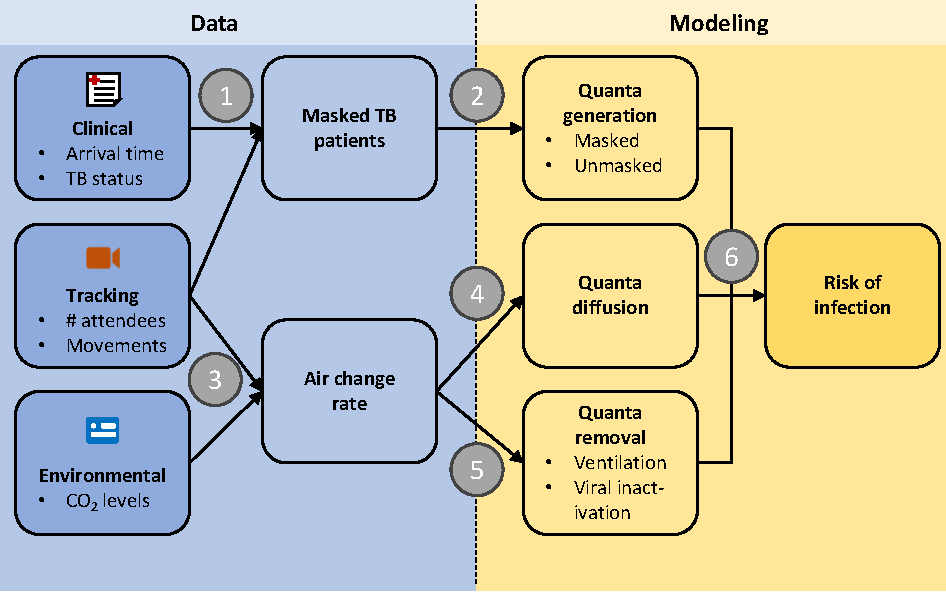
\includegraphics{doc/paper/flow-chart.pdf}
    \caption{Flow chart of the spatiotemporal modeling approach illustrating the steps from data (blue) to modeling (yellow).}
    \label{fig:modeling-flow}
\end{figure}

We divide each separate area of the clinic (waiting room, corridor, TB room) into a grid of cubic cells with an area of 0.25m$^2$ and a volume depending on the height of the room (waiting and TB room: 3m; corridor: 2.5m). We update the quanta concentration every second and assume that $N_{s,0} = 0 ~~ \forall s$, \ie all quanta from the previous day has been removed from the air before the start of the following clinical day. Due to mask wearing, we assume that the initial spread of quanta before diffusion is limited to the cell where the infectious individual is located. We model all model parameters with prior distributions and perform Monte-Carlo simulation to estimate the risk of infection. In each simulation, we perform the following three steps: (i)~sampling uncertain modeling parameters and undiagnosed TB patients, (ii)~computing the spatiotemporal quanta concentration, and (iii)~computing the cumulative risk of infection for each clinical attendee. The model setup, including the specific assumptions and prior distributions, is described in detail in Text~\zref{sec:estimation} in \supp.


\subsection{Statistical analysis}

We analyzed the time-varying CO$_2$ levels, the daily number of registered and masked TB patients, and the number of clinic attendees monitored through patient tracking. We perform 10,000 Monte Carlo simulations and show the average quanta concentration by daytime and summarize the risk of infection with the mean and 95\%-credible interval (CrI) across simulations. To demonstrate the impact of spatial modeling, we compare our modeling approach with one that assumes a well-mixed airspace (\ie where the initial quanta concentration is the same everywhere in the room regardless of where it was generated). Furthermore, we assess the correlation between the personal risk of infection and characteristics of the clinical visit (time spent in each area, number and duration of close contacts). To assess the effectiveness of mask wearing, we compare our modeling results with a scenario where there is no reduction in the generated quanta and the initial spread is extended to the first-neighbouring cells of where the infectious individual is located. All analyses were performed in R software (version 4.3.1)\cite{RCoreTeam2023}.


\subsection{Ethics statement}

The University of Cape Town Faculty of Health Sciences Human Research Ethics Committee (HREC/REF: 228/2019), the City of Cape Town (Project ID: 8139), South Africa, and the Ethics Committee of the Canton of Bern (KEK/REF: 2019-02131), Switzerland, approved the study.

\newpage

\section{Results}

Over the five study days, 894 patients have been registered in the clinical database, of which seven patients were diagnosed with TB and 28 patients were suspected of TB following symptom screening (\supp~Figure~\zref{fig:clinical-data}). Overall, 1,701 unique patient movements were identified after processing the video sensor data. Most patient movements were detected in the waiting room (\Cref{fig:input-data-descriptives}a) and during the morning (\Cref{fig:input-data-descriptives}b). Clinical attendees spent spend around half an hour in the clinic (median 24 minutes, interquartile range [IQR] 12$-$45), and several attendees spent more than an hour in the clinic, most of it in the waiting room (\Cref{fig:input-data-descriptives}c). During their visit, close contacts, defined as an interaction with another attendee within 1m for more than 1min, were frequent (median 5, IQR 2$-$9), and several attendees had more than 10 close contacts (\Cref{fig:input-data-descriptives}d). The majority of clinical attendees was in close contact with at least one other attendee for more than half the time of their visit (median 68\%, IQR 41\%$-$87\%, \Cref{fig:input-data-descriptives}e). The CO$_2$ levels inside the clinic were low, peaking at only about 600\,ppm in the morning (\Cref{fig:input-data-descriptives}f). Based on room size, time-varying occupancy, and CO$_2$ levels, the estimated air change rates indicated that the clinic was well-ventilated, especially the waiting room (median 29 air changes per hour, IQR 9$-$36) and corridor (median 28, IQR 16$-$36), with lower rates in the less frequently occupied TB room (median 6, IQR 5$-$12, \Cref{fig:input-data-descriptives}g). 


\begin{figure}
    \centering
    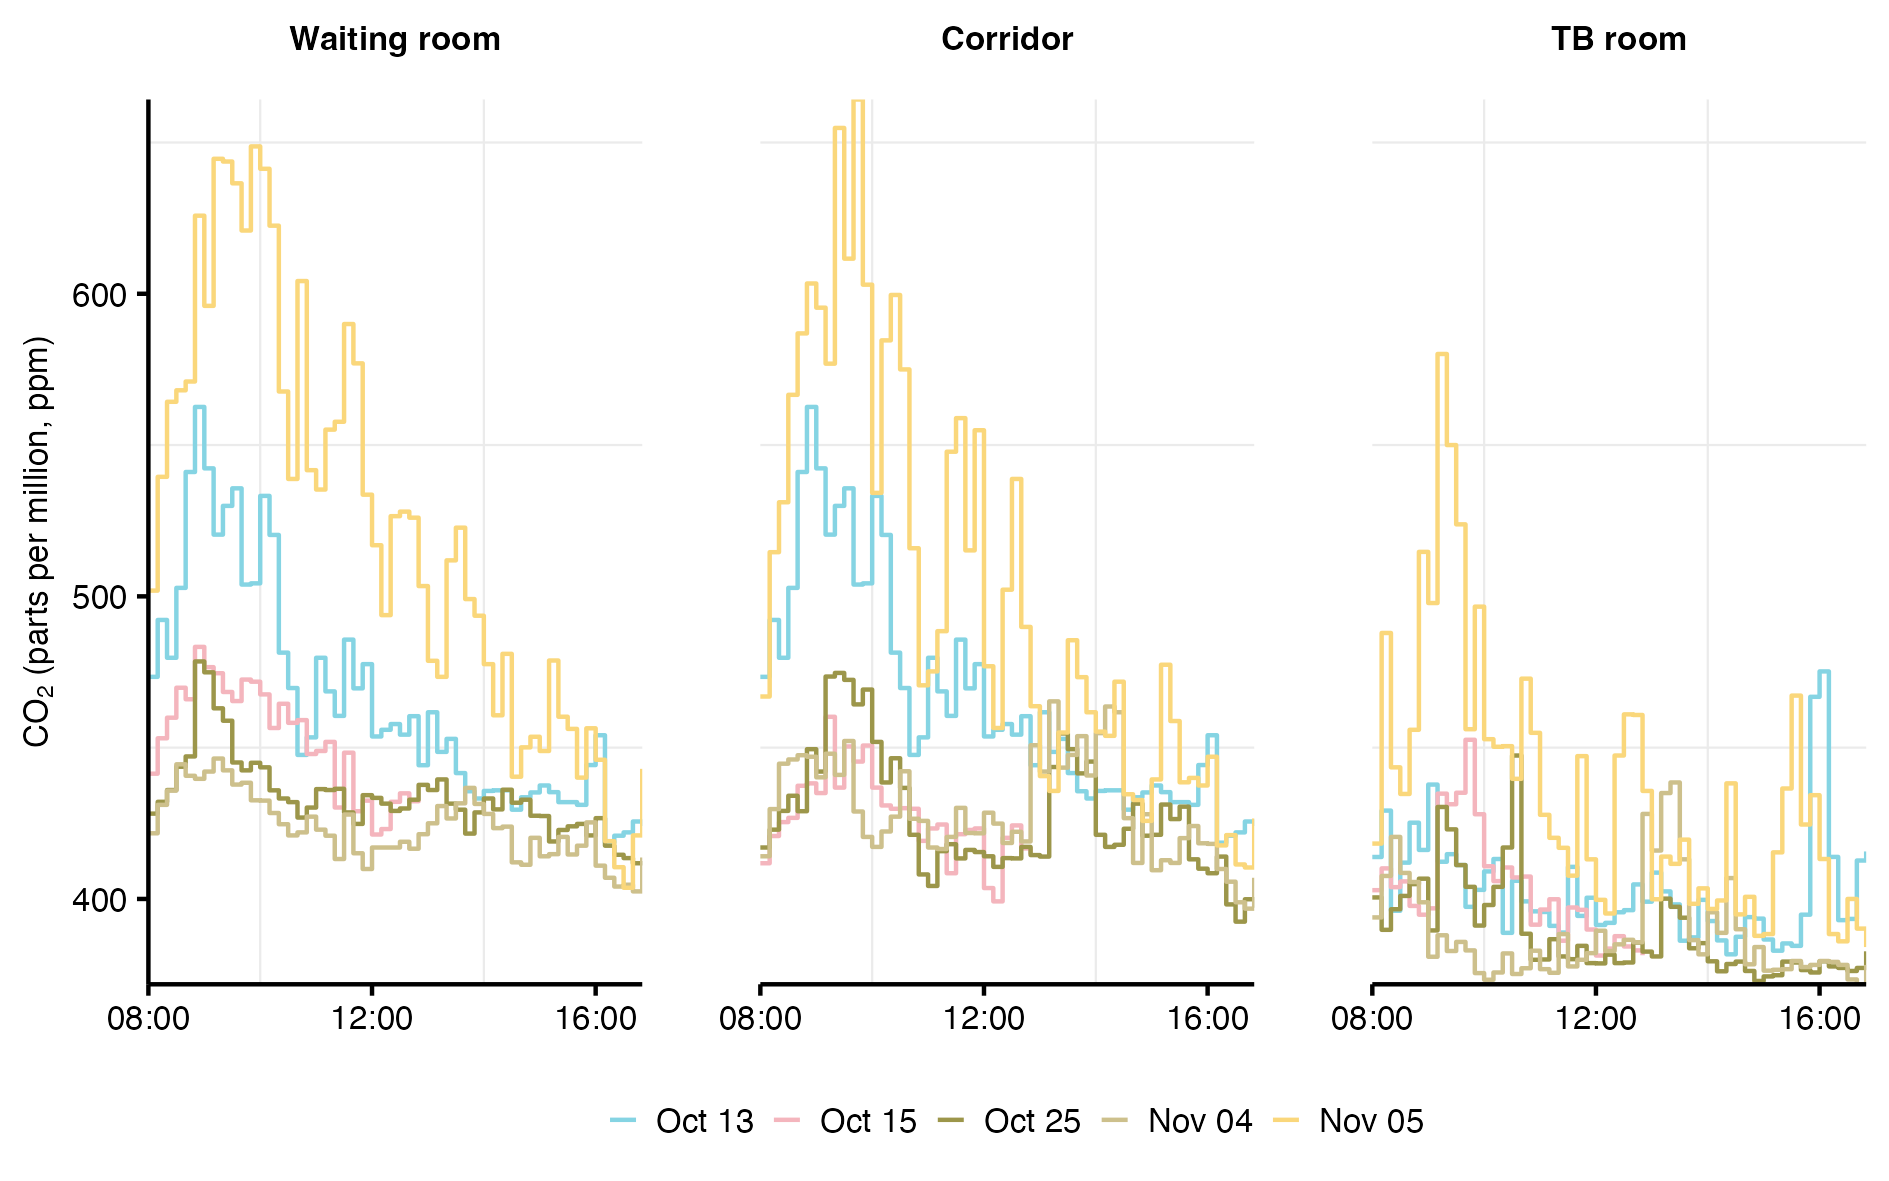
\includegraphics{results/data/co2-levels-over-time.png}
    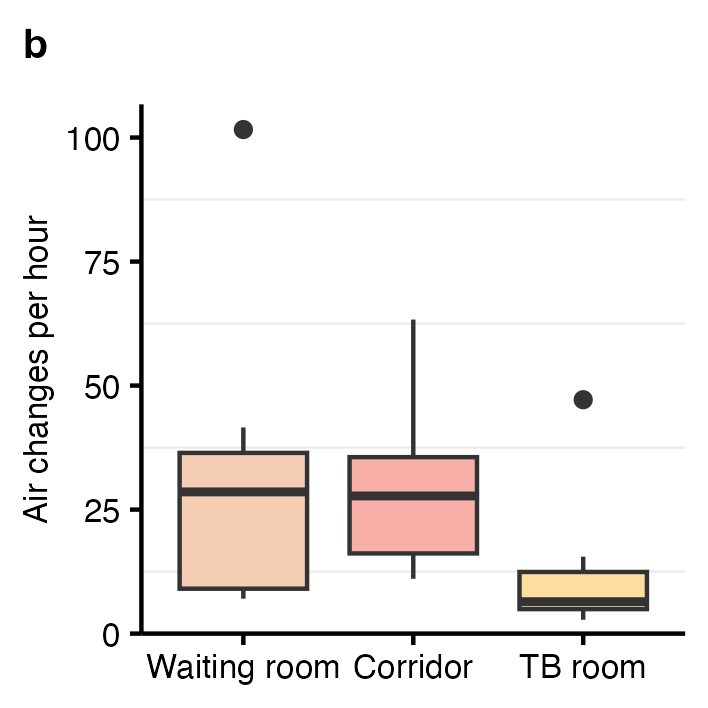
\includegraphics{results/data/air-changes-per-hour.png}
     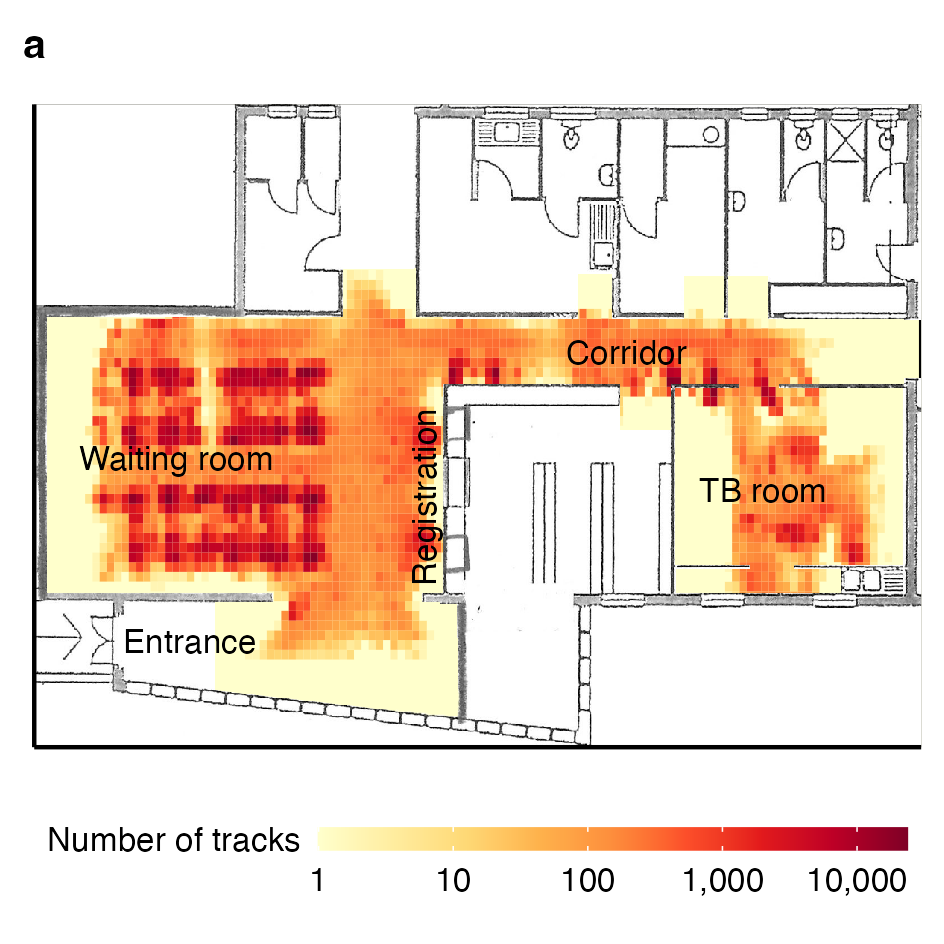
\includegraphics{results/data/no-people-spatial.png}
    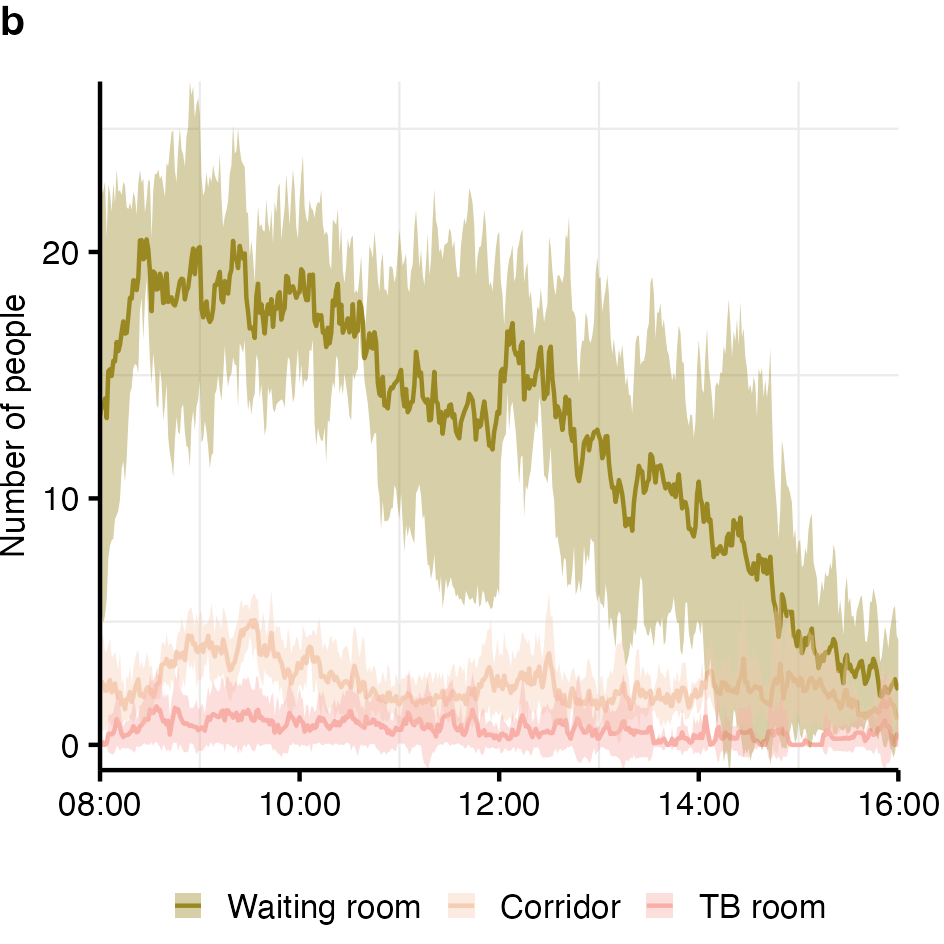
\includegraphics{results/data/no-people-over-time.png}
    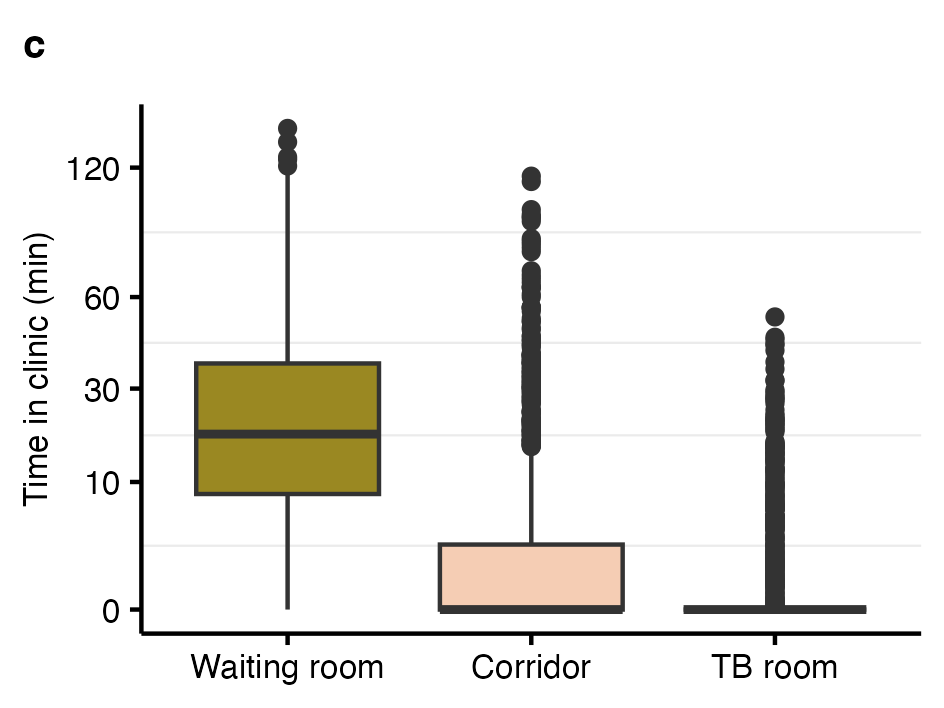
\includegraphics{results/data/time-in-clinic.png}
    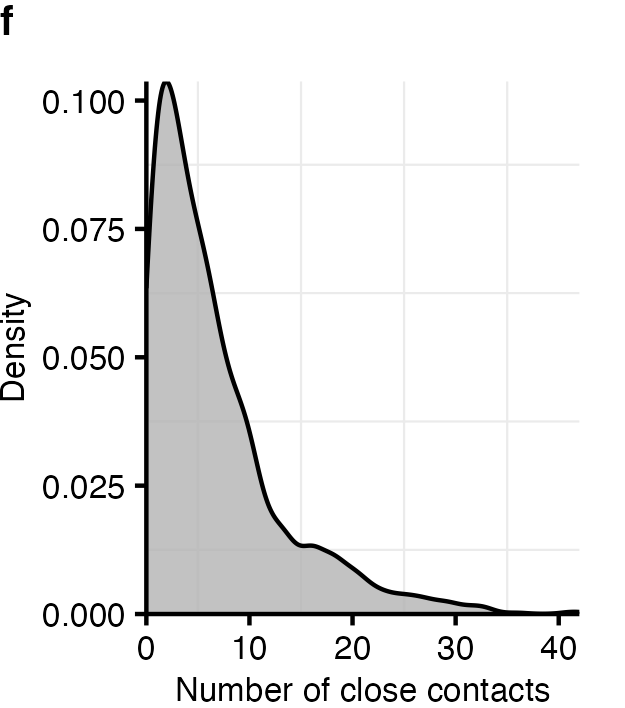
\includegraphics{results/data/number-close-contacts.png}
    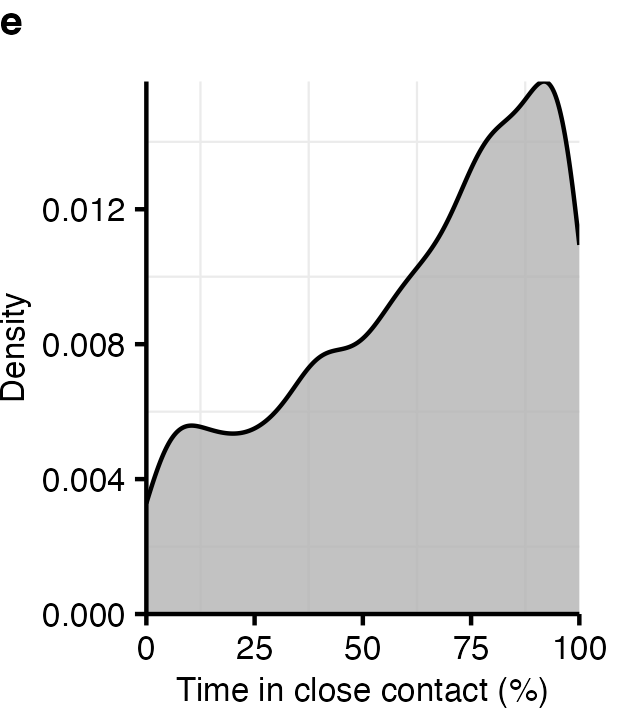
\includegraphics{results/data/time-close-contacts.png}
    \caption{\textbf{Environmental conditions and patient movement characteristics.} \textbf{(a)}~CO$_2$ levels per room of the clinic over time per day. \textbf{(b)}~Air change rates per room of the clinic. \textbf{(c)}~Total number of tracks recorded per unit space in the clinic over the study period. \textbf{(d)}~Number of people in the clinic over time per day. \textbf{(e)}~Time spent in the clinic per clinical attendee. \textbf{(f)}~Density distribution of the number of close contacts per clinical attendee during their visit. \textbf{(g)}~Density distribution of the time spent in close contact per clinical attendee during their visit.}
    \label{fig:input-data-descriptives}
\end{figure}

\begin{figure}
    \centering
    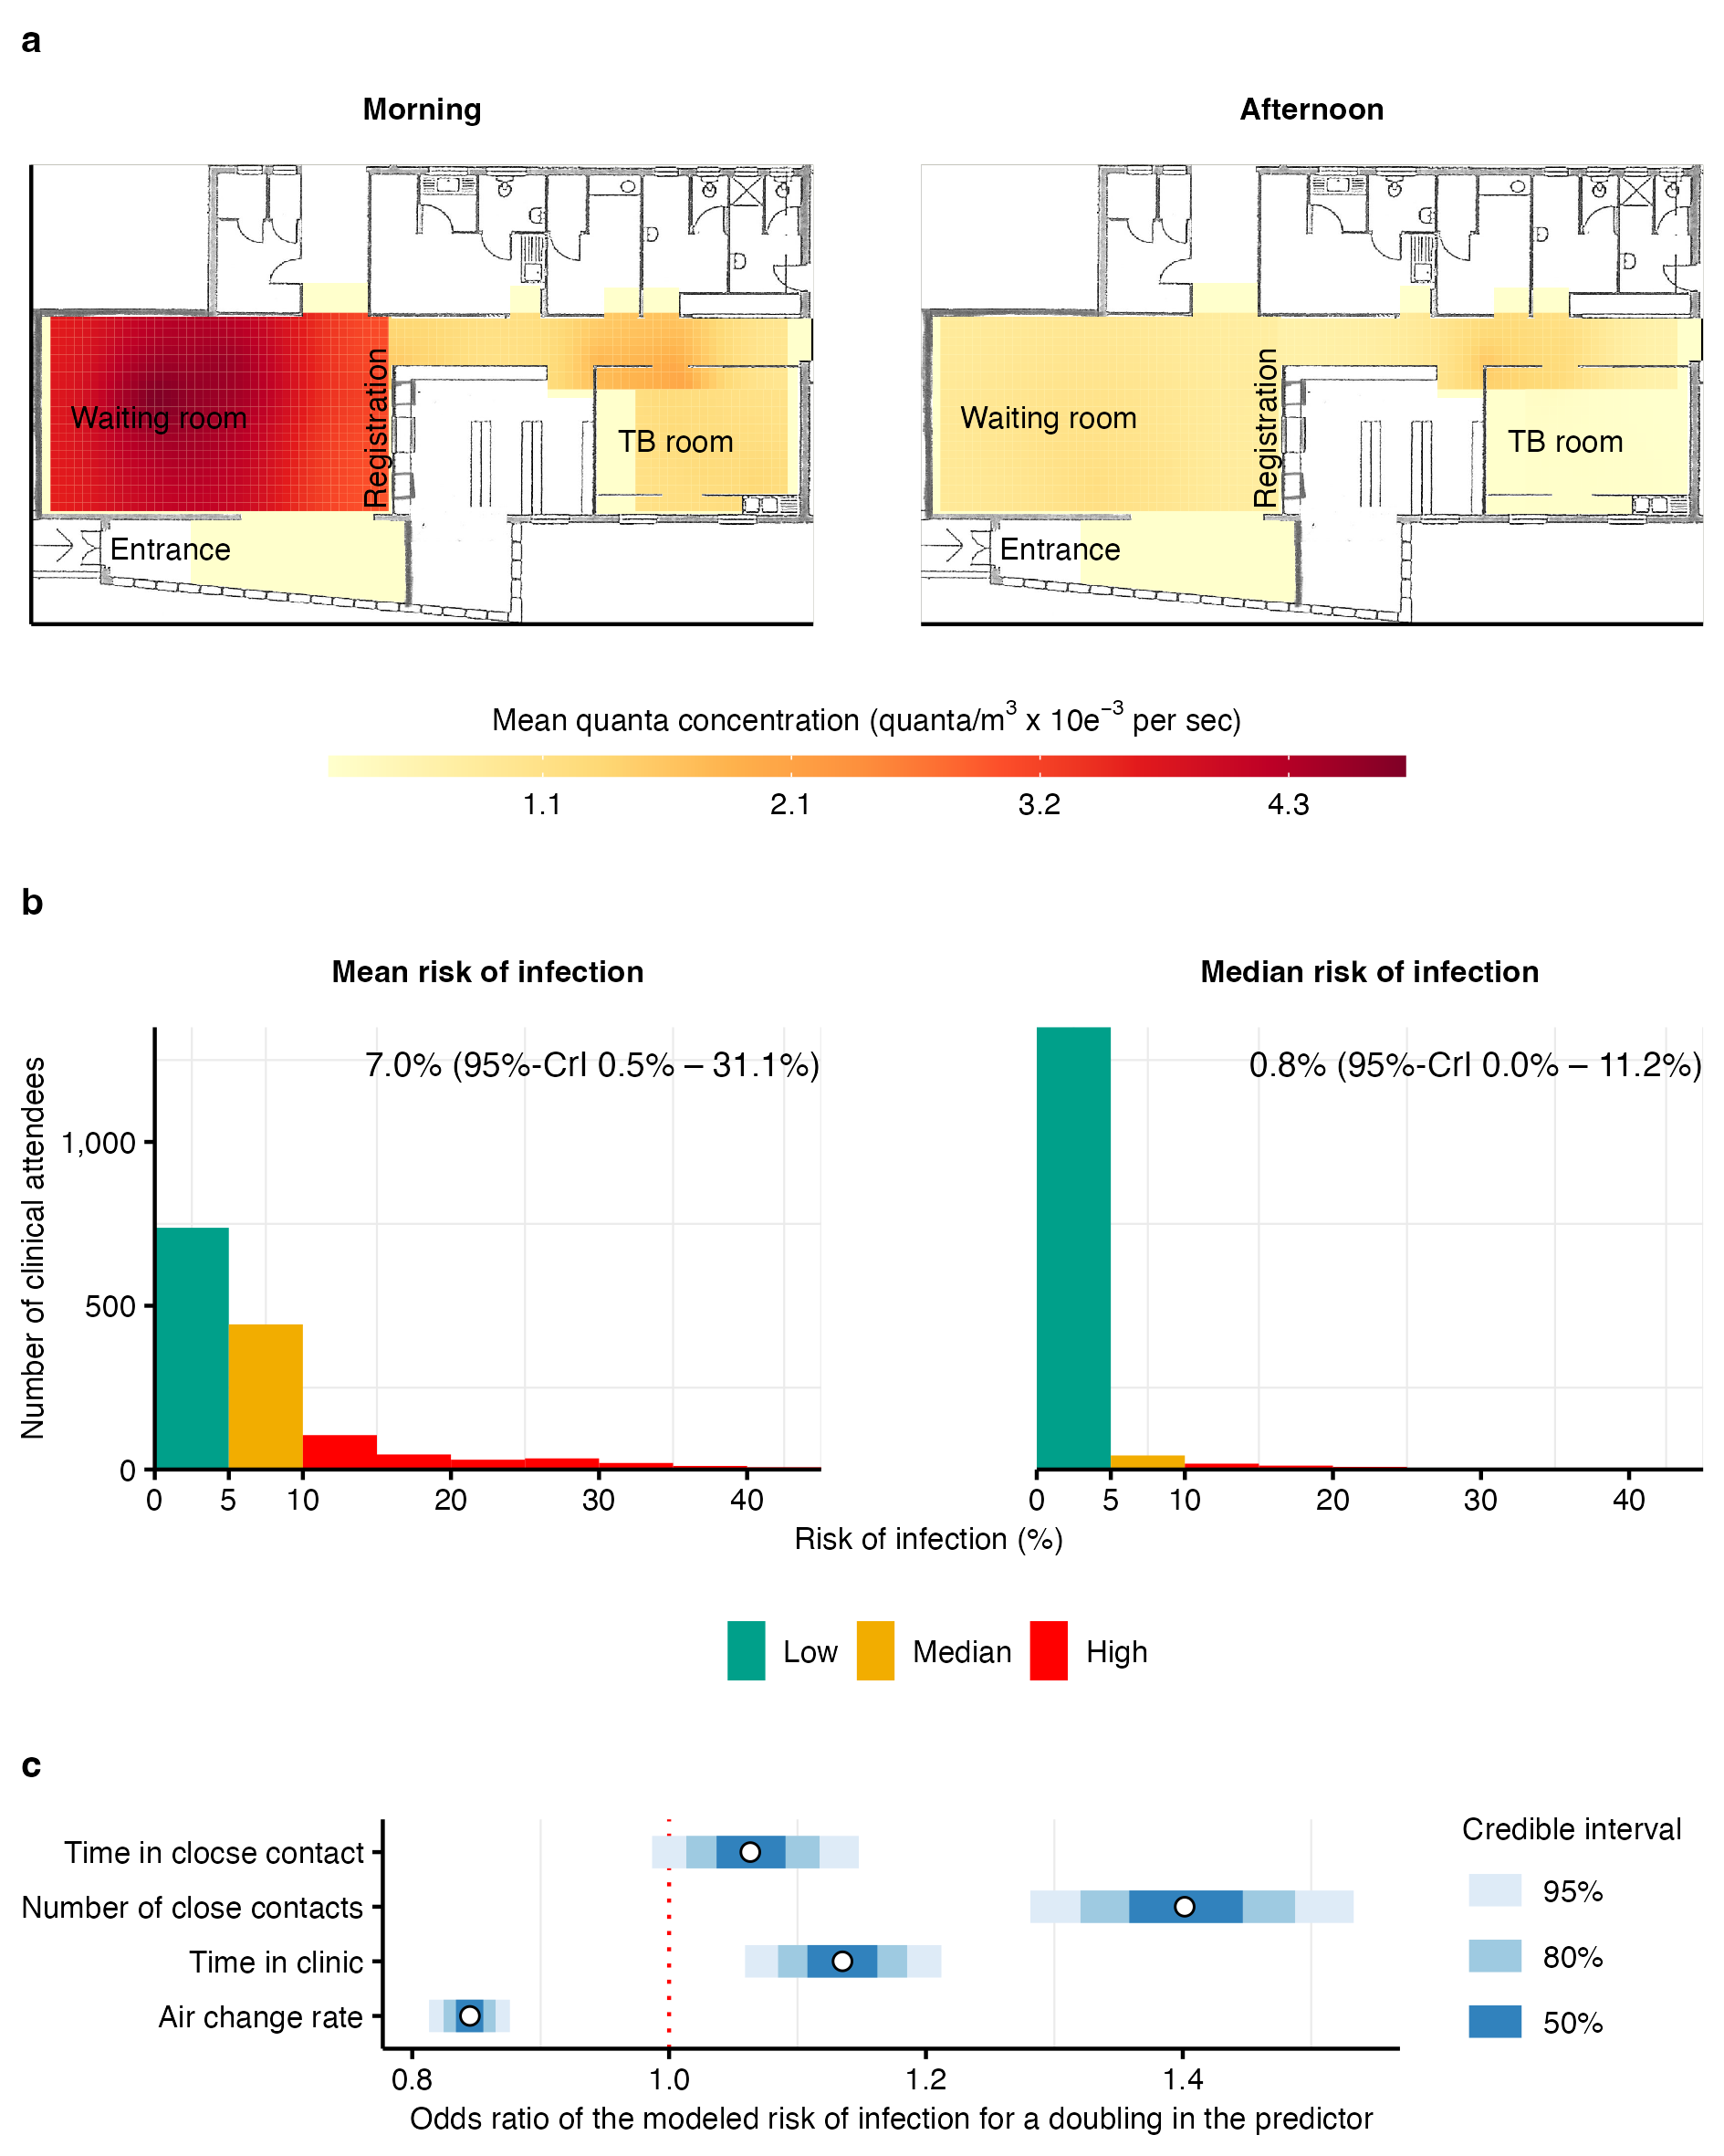
\includegraphics{results/modeling/main-figure.png}
    \caption{\textbf{Spatiotemporal modeling results.} \textbf{(a)}~Average quanta concentration in the morning and afternoon in the clinic. \textbf{(b)}~Mean and median risk of infection per clinical attendee. Low: <5\%, Medium: 5-10\%, High: >10\%. \textbf{(c)}~Association of mean infection risk with patient movement characteristics and environmental conditions. }
    \label{fig:main-modeling-results}
\end{figure}

\begin{figure}
    \centering
    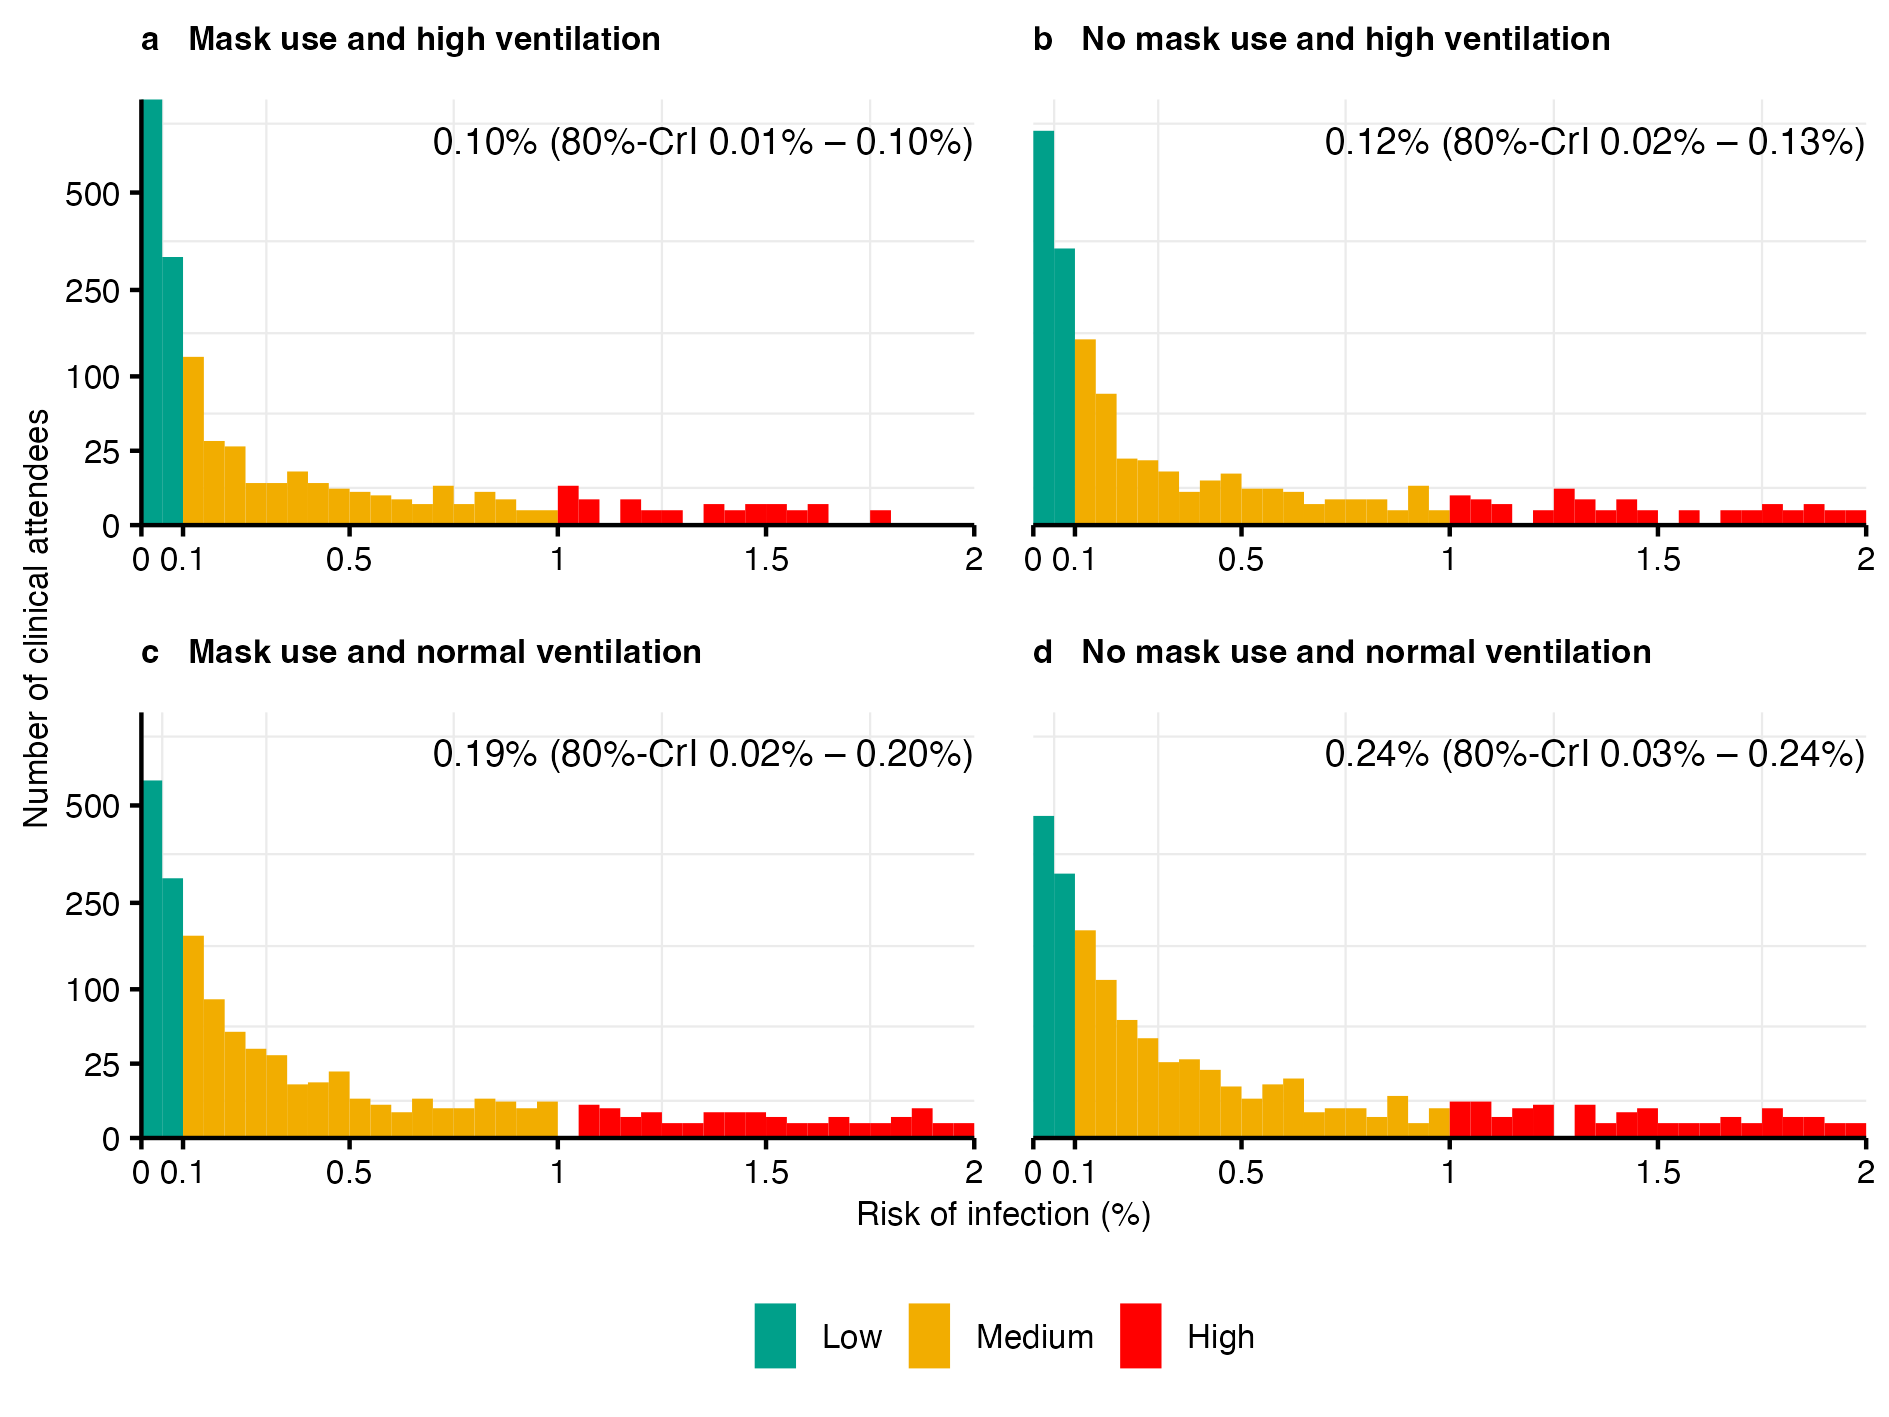
\includegraphics{results/modeling/mean-roi-comparison.png}
    \caption{\textbf{Scenario modeling results.} Mean risk of infection per clinical attendee if \textbf{(a)}~masks had not been worn by all clinical attendees and staff, \textbf{(b)}~the ventilation rate had been lower as in the year before the COVID-19 pandemic, \textbf{(c)}~the number of infectious people in the clinic corresponded to the prevalence of TB in the population, or \textbf{(d)}~the number of infectious people in the clinic corresponded to the number of diagnosed TB patients and those suspected of TB due to respiratory symptoms when attending the clinic. Low: <5\%, Medium: 5-10\%, High: >10\%.}
    \label{fig:scenario-results}
\end{figure}


\FloatBarrier

\newpage

\section{Discussion}

% summary
We modeled the spatiotemporal concentration of infectious quanta, considering the location of infectious individuals (quanta generation), spatial dispersion (quanta diffusion), and natural ventilation (quanta removal). We found ... 


% critical appraisal of our results


% close contacts
Our spatiotemporal model can be viewed as a modified version of the original Wells-Riley transmission model\cite{Riley1978AJE}. It is motivated by previous findings that prolonged close contact is required for transmission\cite{Leung2020NatMed,Brankston2007LancetID,Narasimhan2013PulmonaryMed}. As a result, our model assigns a higher risk of infection to clinical attendees that spend more time in close proximity to infectious individuals. It could thus be used to assess the effectiveness of interventions targeting a reduction in the number of close contacts. Although such assessments only show the potential (modeled) impact of interventions, they can still provide a first estimate about how contact reductions translate into lower transmission risks in crowded indoor settings. Nevertheless, we acknowledge that transmission events are generally difficult to predict. Their occurrence depends on many other factors such as airflow, the properties of the pathogen, and variation in infectiousness of the source and susceptibility of the host\cite{Wang2021Science}. We discuss these factors in more depth in Supplementary Text~\zref{sec:depth-discussion} in \supp.

% more complex models and our relation
An important factor that is omitted from our model is airflow. Poor ventilation settings can generate an airflow where infectious particles circulate rather than being dispersed and removed from the indoor space\cite{Li2021BuildEnv}. There is large stream of literature considering airflow using computational fluid dynamics (CFD) models to simulate the spatial spread of infectious aerosols in indoor environments, \eg Ref. \cite{Vuorinen2020SafSci,Jung2021InfectChemo,Li2021BuildEnv}. CFD models can also be combined with the Wells-Riley model to estimate the risk of infection\cite{Yan2023BE,Qian2009BE,Li2022SOTTE}, thus are seemingly appealing to our setting as well. However, because they are computationally expensive, CFD models are often only used for experiments, short simulations, and static environments. They also require detailed knowledge about the indoor space, in particular airflow, to model particle transport. By contrast, our setting presents a dynamic environment with frequent patient movements over multiple days in a naturally ventilated space (varying airflow). Moreover, we run our model multiple times in a large number of Monte Carlo simulations to consider uncertainty in all modeling parameters and unmasked infectious TB patients. 



% conclusions
We conclude ...


\newpage


%TC:ignore
\section*{Acknowledgements}
...

\bibliography{references.bib}
%TC:endignore

\end{document}
